\documentclass[11pt]{article}
\usepackage{graphicx} % Required for inserting images
\usepackage[top=2.5cm, bottom=2.5cm, left=2cm, right=2cm]{geometry}
\usepackage[T1]{fontenc}
\usepackage{wrapfig}
\usepackage{hyperref}
\usepackage[utf8]{inputenc}
\usepackage{multirow}
\usepackage{subcaption}
\usepackage{booktabs}
\usepackage{bookmark}
\usepackage{graphicx}
\usepackage{setspace}
\usepackage{listings}
\usepackage{xcolor}  % Opcional, per colors
\lstset{
  language=Python,
  basicstyle=\ttfamily\small,
  keywordstyle=\color{blue},
  commentstyle=\color{gray},
  stringstyle=\color{green!50!black},
  showstringspaces=false,
  numbers=left,
  numberstyle=\tiny\color{gray},
  frame=single,
  breaklines=true,
  captionpos=b,
  tabsize=4
}

\setlength{\parindent}{0in}
\usepackage{physics}
\usepackage{tikz}
\usepackage{tikz-3dplot}
\usepackage[outline]{contour} % glow around text
\usepackage{xcolor}
\usepackage{float}
\usepackage{makeidx}
\usepackage{fancyhdr}
\usepackage{pgfplots}
\usepackage{amsmath}
\pgfplotsset{compat=1.18}
\usepackage{caption}
\usepackage[english,catalan]{babel}
\setlength{\parskip}{11pt}
\usepackage{xcolor}
\usepackage{listings}
\usepackage{marginnote}
\usepackage{siunitx}
\usepackage{framed}
\usepackage{ulem}

\numberwithin{equation}{section}
\numberwithin{figure}{section}
\numberwithin{table}{section}

\begin{document}
\tableofcontents
\newpage
\vspace{10em}

{\huge \textbf{Pràctica 2}}  % Títol petit en negreta

\vspace{0.5em}  % Espai vertical

{\Huge \textbf{Força entre corrents}}  % Títol gran

\vspace{1em}  % Espai abans del contingut

\begin{abstract}
    En aquesta pràctica estudiem la força magnètica entre dos fils amb corrent elèctric de mateixa intensitat, en concret, analitzem la seva relacció amb la magnitud d'intensitat dels fils i la dependència amb la distància que els separa. També s'aprofita el muntatge experimental per mesurar la component horizonal del camp magnètic terrestre. Les dades experimentals es tracten mitjançant el mètode dels mínims quadrats per obtenir paràmetres que es poden comparar amb valors teòrics. Aquests presenten diferències prou significatives respecte els nostres resultats tot i trobear-se dins l'interval d'incertesa, el que creiem que és degut a la gran complexitat del mètode experimental emprat.
\end{abstract}

\section{Introducció}\label{sec: PR2_intro}

En aquesta pràctica tenim per objectiu estudiar la força magnètica que es genera entre dos fils pels quals es fa passar corrent elèctric. També, aprofitarem el muntatge experimental per a mesurar la component normal del camp magnètic terrestre.

La força magnètica entre dos fils finits de corrent es calcula a través de la llei de Biot-Savart. Però tenint que la separació entre els fils de corrent és molt menor a la longitud d'aquests, podem arribar a considerar que el camp magnètic que rep un dels fils és el generat per un altre fil infinit situat a una distància d'ell. 

Aquesta aproximació ens facilita molt més els càlculs ja que podem trobar el camp magnètic generat per un fil infinit amb la llei d'Ampère, que ens dona com a resultat la següent expressió:

\begin{equation}\label{eq_PR2: PR2_camp_fil_infinit}
    B = \frac{\mu_0I}{2\pi r}
\end{equation}

I que la força mangètica que rep el fil d'una longitud $L$ és

\begin{equation}\label{eq: PR2_Fmagn_en_funcio_B}
    \vec{F} = I\oint d\vec{l}\times\vec{B}(\vec{r})
\end{equation}

Ens resultat que la força magnètica (el mòdul) té l'expressió següent:

\begin{equation}\label{eq: PR2_Fm_entre_fils}
    F = \frac{\mu_0I^2L}{2\pi r}
\end{equation}

Per mesurar la força magnètica entre dos fils de corrent i la seva dependència amb la intensitat de corrent que hi circula i amb la distància de separació entre ells utilitzarem una balança. Aquesta permet saber quan el sistema està en equlibri, és a dir, quan la força magnètica generada pels fils és compensada per una altra força d'igual direcció però sentit contrari. 

Aquesta altra força, que ha de ser fàcilment parametritzable, pot correspondre a la força gravetat  associada al fil superior. La qual mesurarem a través de les masses conegudes que col·locarem sobre la cassoleta que té aquest fil.

També pot correspondre a la força de torsió del sistema que conté el fil superior. La qual es pot mesurar a través de l'angle de gir resultant del fil superior al rebre la força magnètica.
 
La força gravetat segueix la següent equació

\begin{equation}\label{eq: PR2_Fgrav}
    F_{grav} = mg
\end{equation}

I la força de torsió

\begin{equation}\label{PR2_Ftorsio}
    F_{tor} = k\theta
\end{equation}

\section{Mètode Experimental}\label{sec: PR2_met_exp}

La balança de corrent està formada per un marc rectangular per on hi circula un corrent, gr. Aquest es troba sustentat pel fil de torsió i es troba sotmès a un equilibri entre la força del contrapes i la força entre fils. 

Per tal d'afavorir el moviment del rectangle conductor, les
connexions entre el marc i la font de corrent es fan usant gal·li fos. Els motius pels quals s'usa el gal·li són la seva baixa temperatura de fusió (29;76ºC) i al seu preu econòmic. El metall fos permet la mobilitat del marc i proporciona una connexió continua i gairebé sense presentar fricció. S'obren els pots de gal·li i es connecta el transformador de corrent de 9 V per fondre'l. 

A continuació, es posen en contacte
els pots de gal·li amb el marc rectangular, que té unes petites puntes sobresortint que entre perfectament en l'obertura de cada pot de gal·li. També es connecta el transformador amb el fil inferior, per a que aquest també tingui corrent circulant-hi.

%DIBUIX MUNTATGE

\begin{figure}[H]
    \centering
    \begin{subfigure}{0.4\textwidth}
        \centering
        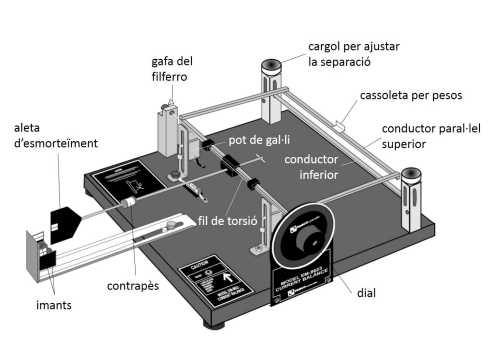
\includegraphics[width=0.5\textwidth]{PR2_dib_muntatge_parts.jpg}
        \caption{Parts de la balança usada en l'experiment.}
        \label{fig: PR2_dib_muntatge_parts}
    \end{subfigure}
    \hspace{0.1\textwidth}
    \begin{subfigure}{0.4\textwidth}
        \centering
        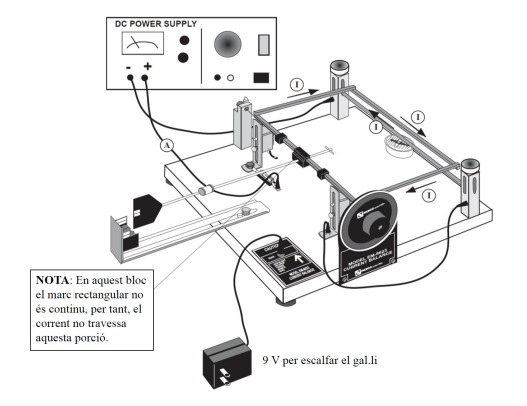
\includegraphics[width=0.5\textwidth]{PR2_dib_muntatge_corrent.jpg}
        \caption{Connexions per a fer circular corrent pels fils de la balança.}
        \label{fig: PR2_dib_muntatge_corrent}
    \end{subfigure}
\caption{Muntatge de la balança usada}
\end{figure}

La importància de la presa de mesures en aquesta pràctica recau en la calibració de la balança. Primerament, es col·loca la balana de tal forma que els cables siguin paral·lels al camp magnètic terrestre, seguint la direcció que ens indica la brúixola. Així, es pot eliminar la contribució del camp
magnètic terrestre, que alteraria els resultats. 

En segon lloc ajustem les potes de les potes de tal manera que la bombolla quedi al centre de l'espai disponible que te per moure's, fet que indica que està completament paral·lela al pla z. A continuació, ens assegurem que el dial de torsió del marc rectangular està al zero. 

Finalment, es mou el contrapès fins que la balança estigui estable i després es mou el cursor de marques, que conté uns imants per disminuir l'oscil·lació de l'aleta d'amortiment fins que ens quedin alineades amb la marca de l'aleta.

Després de fer una mesura, la balança pot quedar descalibrada (l'aleta d'amortiment no queda alineada amb el cursor de marques). Si aquest és el cas, cal tornar a calibrar la balança de nou.

Un cop la balança calibrada, la pràctica es divideix en 3 parts. En la primera part, es fan girar els cargols 5 voltes completes de tal forma que se separen els cables 5 mm més. A continuació es posa la massa de 5 mg i es connecta la font de corrent continu augmentant la intensitat ens que
s'equilibra la balança. Es repetirà el mateix procés per a les diferents masses, augmentant-les de 5 mg en 5 mg.

En la segona part de la pràctica, es posa la massa de 5mg sobre la cassoleta i es gira el dial ens que la balança torni a l'equilibri. Seguidament es repeteix el procés per les masses de 10, 15, 20 i 25 mg i a continuació es van separant els fils a I constant (girant les rodetes que desplacen el fil inferior) per a trobar el valor de $\mu_o$.

Finalment, en la tercera part de la pràctica es rota el sistema 90 graus per així detectar la component normal del camp magnètic terrestre. A continuació, es desconnecta la intesitat del cable inferior i pel superior es fa circular la major intensitat possible. Finalment, es gira el dial fins a equilibrar la balança.

%EQUILIBRAT DE LA BALANÇA

Per saber si el sistema es troba en equilibri cal fixar-nos en que les 3 línies, les dues del cursor de marques i la de l'aleta d'amortiment es trobin perfectament alineades. 

\iffalse
DIBUIX LLENGUETES
\begin{figure}[H]
    \centering
    \includegraphics[width=0.5\textwidth]{PR2_dib_llenguetes.jpg}
    \caption{Posició de les llenguetes quan balança està en equilibri.}
    \label{fig: PR2_dib_llenguetes}
\end{figure}
\fi

A la pràctica, l'aleta d'amortiment mai es quedava en una posició sense moviment. Així doncs, preniem com sistema en equilibri vàlid per a la mesura quan l'aleta patia la mínima osicil·lació possible, d'amplitud constant (igual desplaçament amunt i avall).

\section{Presentació i discussió de resultats}\label{sec: PR2_resultats}

\subsection{Dependència de la força mangètica amb la intensitat de corrent}\label{sec: PR2_Fm_intensitat}

En la primera part de la pràctica volem estudiar la relació que hi ha entre la intensitat que circula per un fil i la força que aquest rep a causa d’un altre fil pel que hi circula la mateixa intensitat. 

S’ha mesurat la intensitat necessària per fer circular pel fil perquè la força magnètica i la força gravitatòria de la massa de la balança estiguin en equilibri. S’ha fet la mesura per a 5 masses diferents, començant per 5 mg, i augmentant-la de 5 en 5 mg a cada nova mesura. Per a cada massa s’han
realitzat 3 mesures de la intensitat i se n’ha fet el promig.

Per comprovar la dependència s’ha representat la força en funció del quadrat de la intensitat i s’ha fet una regressió lineal. Els
valors obtinguts es mostren gràficament a la Fig. \ref{fig: regr_mvsI2}:

\begin{figure}[H]
    \centering
    \includegraphics[width=0.5\textwidth]PR2_regr_I2vsF.png}
    \caption{El quadrat de la intensitat en funció de la Força.}
    \label{fig: PR2_regr_I2vsF}
\end{figure}

La regressió té un coeficient de correlació de $R^2 = 0,98$. Axií doncs, que la força que un fil que transporta una intensitat I rep a causa d’un altre fil que transporta la mateixa intensitat I compleix la lineal proporcional: $F \sim I^2$.

El pendent de la recta de regressió ens permet trobar un valor aproximat de $\mu_0$. A partir de l’Eq. \eqref{eq: PR2_Fm_entre_fils} es dedueix que el pendent m serà $m = \frac{2\pi d}{\mu_0 L}$. Aïllant $\mu_0$ s’obté $\mu_0 = (0,413 \pm 0,091) · 10^{-6}$ T · m/A, que difereix bastant (tot i tenir el mateix ordre de magnitud) del valor real que hem pres, de $4\pi · 10^{−7}$ T · m/A $= 1,26 · 10^{−6}$ T·m/A. 

Podem veure que el valor teòric no es troba dins l’interval d’incerteses considerat pel valor experimental i per tant els resultats no són compatibles. La incertesa instrumental associada a les mesures com per exemple la diferència de massa real respecte el marcat en les etiquetes i el que s'ha utilitzat per fer les regressions fa augmentar la discrepància entre els resultats. 

\subsection{Dependència de la força mangètica amb la distància de separació entre fils}\label{sec: PR2_Fm_sep}

En aquest segon apartat analitzarem com depèn la força magnètica amb la distància de separació entre fils per on circula corrent. 

Ho farem aconseguint mantenir en equilibri la força magnètica amb la força de torsió. Així doncs, primer cal obtenir la constant de torsió del fil. Es fixa una intensitat de (5,00 ± 0,01)A i es representen les dades de la força en funció de l’angle. Posteriorment es realitza una recta de regressió que ens permet trobar el valor de la constant k.

\begin{figure}[H]
    \centering
    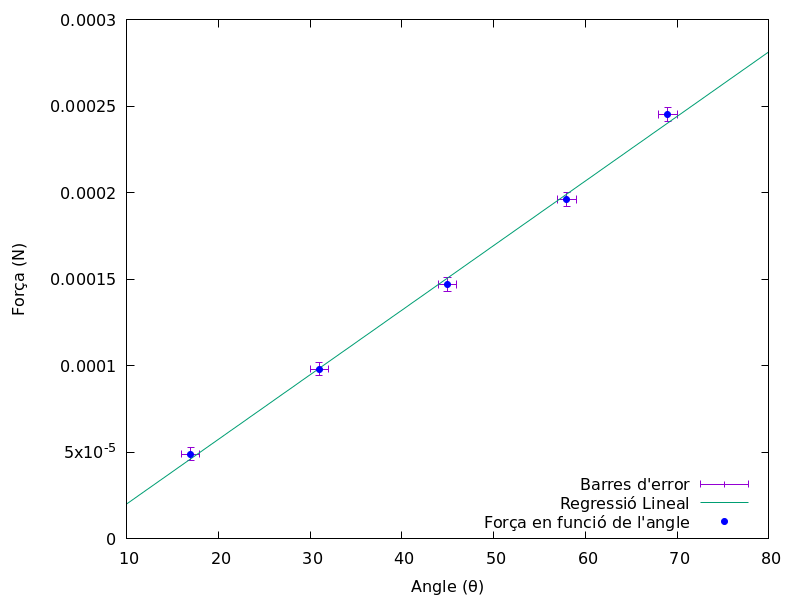
\includegraphics[width=0.5\textwidth]{PR2_regr_Fvstheta.png}
    \caption{Força en funció de l'angle de torsió.}
    \label{fig: PR2_regr_Fvstheta}
\end{figure}

La força que s’obté de la regressió és:

\begin{equation}\label{F_ktheta}
    F(\theta) = (3,73 \pm 0,10) · 10^{-6}\theta
\end{equation}

Cal remarcar que la regressió lineal posseeix una ordenada a l’origen llunyana al zero ($(-1,75 \pm 0,50)·10^{-5}$). Tot i que aquesta ordenada d’origen no és menyspreable enfront els valors de la força,\textbf{ els resultats experimentals avalen que es pot no tenir en compte}. Aquesta ordenada d'origen pot haver aparegut a causa d’una imprecisa cal·libració de la balança, ja que es feia a ull. A més a més, el fet que la constant sigui positiva és un bon indicatiu, perquè la força ha d’augmentar linealment amb l’angle de torsió.

A continuació, mantenint fixa la intensitat anterior, es va variant la distància entre ambdós fils de corrent per calcular el valor de la permeabilitat magnètica $\mu_0$. 

Es representen els resultats obtinguts en la Fig. \ref{fig: PR2_regr_thetavsr} on es grafica la força respecte 1/r:

\begin{figure}[H]
    \centering
    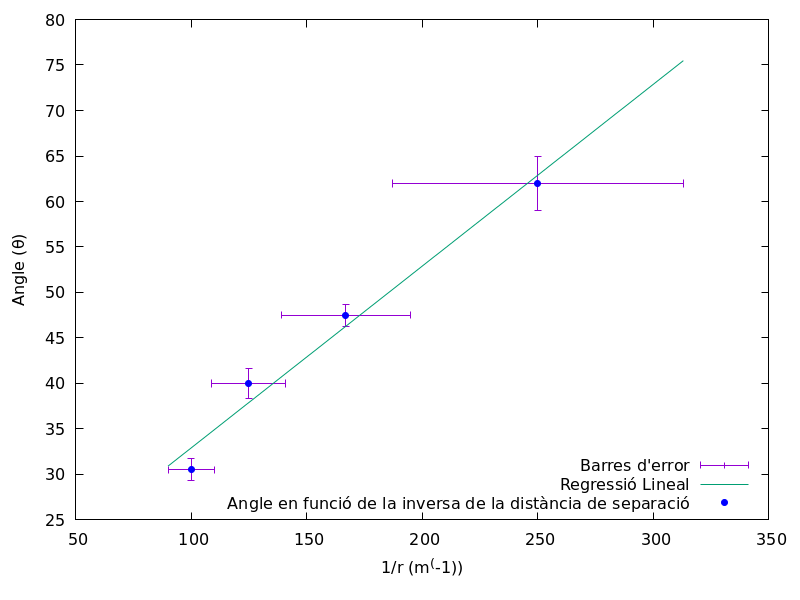
\includegraphics[width=0.5\textwidth]{PR2_regr_thetavsr.png}
    \caption{Força en funció de l’invers de la distància de separació entre fils de corrent.}
    \label{fig: PR2_regr_thetavsr}
\end{figure}

La regressió té un coeficient de correlació de $R^2 = 0,976$.
Aplicant la relació \eqref{F_ktheta} a l'equació que acabem de trobar i operant, s’obté que el valor de $\mu_o$ ve donat per l’equació $\mu_0 = \frac{2πm}{LI^2}$ on $m$ correspon al pendent de la regressió lineal. 

Aplicant el valor experimental s’obté que: $\mu_0 = (0,525 \pm 0,058) · 10^{-6} N/A^2$. Tot i que el resultat tampoc és compatible amb l’esperat, sí és molt similar al resultat experimental de l’apartat anterior (tenint en compte els seus intervals d'incertesa, sí són compatibles) . 

De nou, cal considerar que la discrepància és deguda la complexitat en la mesura de les dades. Un error tan gran pot ser degut a factors que han influït en la mesura i que no s’han pogut tenir en compte en el càlcul de la incertesa, com ara petites vibracions de la taula o una calibració imprecisa de la balança. De fet, tenir aquesta mateixa discrepància en els dos càlculs de la permeabilitat magnètica al buit pot ser un indicatiu que la balança no estava ben calibrada, per això les dependències entre magnituds són correctes però els valors calulcats no. Tanmateix, el resultat és força proper al valor real.

Per millorar l'experiment i que els resultats numèrics fóssin més propers al teòric caldria considerar que la posició d'equilibri es devia trobar desplaçada del zero. També es podria recalibrar la balança de nou per no seguir arrossegant aquest error. Això és el que vam realitzar abans de començar la mesura del camp magnètic terrestre en la secció que ve a continuació.

\subsection{Camp magnètic terrestre}\label{sec: PR2_Bterra}

En aquesta última part de la pràctica es pretén mesurar la component horitzontal del camp magnètic terrestre. Per fer-ho, s’ha girat el dispositiu 90º de manera que sigui el camp de la Terra qui faci la força sobre el fil de corrent (recordem que fins ara el teníem paral·lel al camp de
la Terra perquè aquest no fes cap força sobre el fil). D’aquesta manera, mesurant la força que rep el fil es podrà trobar de quina magnitud és el camp causant d’aquesta força.

Per a una intensitat determinada, la força que rep el fil ve donada per l’equaci´o (2.2), i simmplement a¨ıllant el camp es podria trobar el seu valor. 

Fixant la intensitat a $(8,00 \pm 0,01)A$, trobem el valor de l'angle que permet tornar a deixar a equilibrar la balança, és a dir, igualem la força que rep el fil degut al camp magnètic amb la de torsió. La torsió obtinguda experimentalment és de $(19,5 ± 2,3)º$. 

Aprofitant el resultat de la constant de torsió trobada en la Sec. \ref{sec: PR2_Fm_sep}, podem trobar que la força magnètica que s’ha obtingut és de $F = (7,28 \pm 0,90) · 10^{-5} N$. 

De l’Eq \eqref{eq: PR2_Fmagn_en_funcio_B}, podem aïllar $B$ i obtenir que la component horitzontal del camp magnètic de la Terra al laboratori de la Universitat Autònoma, és $B = (3,08 \pm 0,59)·10^{-5}T$. El valor real que hem agafat és de $B = 2,53·10^{−5} T$ \footnote{Valor obtingut d'un document de la R.S.E.F. on s'havia mesurat la component horitzontal del camp magnètic a Salamanca}. Per tant, com el valor experimental es troba dins l’interval d’incerteses, és compatible amb el resultat esperat.

Només hem pogut estudiar la component horitzontal del camp magnètic terrestre perquè la component vertical d’aquest és perpendicular al conductor i per tant la balança que tenim no permet fer la seva mesura.

També podem observar que el fet d'haver desplaçat la balança, ens ha obligat a recalibrar aquesta de nou. Això pot haver influit en què els resultats de c'alcul del camp magnètic sí continguin el valor teòric en el seu interval d'incerteses.

\section{Conclusions}\label{sec: PR2_concl}

En vista dels resultats es comprova que la dependència en $I^2$ i en $1/r$ de la força magnètica, efectivament és lineal, tal com predien les equacions trobades per un sistema de fils parl·lels pels quals circula una mateixa intensitat. 

També s’ha obtingut experimentalment el valor de $\mu_0$ de dues maneres diferents, obtenint en ambdós casos valors que discrepen amb al valor teòric acceptat però similars entre ells.

Concluim doncs, que el mètode experimental és prou bo tot i els errors que té associats. No obstant, veiem que el calibratge inicial de balança és molt determinant en els resultats numèrics, en el nostre cas, s'hauria de tenir en compte que el punt d'equilibri de la balança es trobava fora del zero o es podria haver recalibrat la balança de nou abans de començar a fer les mesures de cada part de l'experiment.

La component horitzontal del camp magnètic terrestre a la Universitat Autònoma és de $B_{T_{norm}}= (3,08 \pm 0,59)·10^{-5}T$ que conté dins del seu rang d’incertesa el valor teòric mesurat a Salamanca (el qual utilitzem de referència).
